\documentclass[a4paper,10.5pt,twocolumn]{jsarticle}
\usepackage{eshouroku}
\usepackage[dvipdfmx]{graphicx}
\usepackage{amsmath}
\usepackage{url}
\usepackage{here}
\usepackage{booktabs}
\usepackage{remreset}
\usepackage{pdfpages}
\usepackage{comment}
\usepackage{subfigure}
\usepackage{subcaption}
\usepackage{amsmath}

\renewcommand{\subfigtopskip}{2pt}	% 図の上の隙間。上図の副題と下図の間。
\renewcommand{\subfigbottomskip}{0pt} % 図の下の隙間。副題と本題の間。
\renewcommand{\subfigcapskip}{-10pt}	% 図と副題の間
\renewcommand{\subcapsize}{\scriptsize} % 副題の文字の大きさ

\makeatletter
	\renewcommand{\theequation}{% 式番号の付け方
	\thesection\arabic{equation}}
	\@addtoreset{equation}{section}

	\renewcommand{\thefigure}{% 図番号の付け方
	\thesection\arabic{figure}}
	\@addtoreset{figure}{section}

	\renewcommand{\thetable}{% 表番号の付け方
	\thesection\arabic{table}}
	\@addtoreset{table}{section}
\makeatother
%\numberwithin{equation}{section}
%\numberwithin{table}{section}
%\numberwithin{figure}{section}


\boldmaintrue% 主文を太字にするモード(指導教員添削時はこちら)
%\boldmainfalse% 主文を普通文字にするモード(抄録印刷時はこちら)
\graphicspath{{./figs}}
\begin{document}
\twocolumn[
 \講演番号{B-XX}% 必要ない場合には書かない
 \日本語タイトル{\huge}{神経免疫相互作用に着想を得た\\マルチエージェントシステム型ニューラルネットワークの提案}
 \英語タイトル{\large}{Proposal of Neural Network composed of Multi-Agent System Inspired by Nervous-Immune Interaction}
 \筆者一名{5335}{柚木開登}

 \指導教員一名{山本哲也}
 %\指導教員二名{東京花子}{京都紀夫}
 %\指導教員なし
]

%\addcontentsline{toc}{section}{\refname}% 追加

\graphicspath{{./figs/}} % 図が特定のフォルダにある場合には設定

\section{本研究の意義・目的}
\begin{comment}
本来的に大規模な計算資源を必要とするニューラルネットワークが
今日, あらゆる産業へ導入されるに至ったのは, クラウドコンピューティングの貢献がある.
一方で, 同市場拡大に伴って
プラットフォーマによる市場寡占, データセンターでの電力消費, データプライバシーの課題が表面化した.
こうしたクラウドの課題克服に向けて, 
データを集約せずにネットワークの端点(エッジ)で処理するエッジコンピューティングが注目
されている.
\end{comment}
エッジコンピューティングでの機械学習手法として連合学習(Federareted Lerning)が提案されている.
連合学習では, 学習データを集約せずネットワーク中の各ノードで学習し, 
その結果得たパラメータ差分のみを通信し, 平均化することで
大規模な学習済みモデルを構築するため, プライバシーを含んだ学習データは保護される.
機械学習への期待と世界的な個人情報保護の動きの高まりから, 
将来的に連合学習は情報社会において重要な位置を占めることが予測される.

一方, 連合学習の実用化に際しては, 
従来, データセンターで動いていたモデルを計算資源に乏しいエッジ環境に投入する必要があることから
少なくとも以下2点の課題が考えられる.
1つ目は学習パラメータ削減によるモデルの軽量化, 
2つ目は, エッジ環境内の不均一計算資源の利用
である.
前者については刈り込みや, ニューラルアーキテクチャ探索, 後者についてはエージェント志向アーキテクチャによる
分散処理システムや遊休計算資源を用いた大規模分散計算等があり, 
今日までに多様な先行事例・研究が成されている. 
両者を満たしたモデルを構築できれば, 
大規模なニューラルネットワークのエッジ環境への投入を可能にし, 
かつ環境内の計算資源の利用率を最大化することが期待できるが,  
両者を満たしたモデルに関する研究は著者の知る限り存在しない.

そこで本研究では, 将来的に導入が予測されるエッジコンピューティングアーキテクチャ及び, 
それに対応した機械学習手法である連合学習に向けて, 
自律分散性を持ったニューラルネットワークのパラメータ削減を提案する.
提案にあたっては, 生体の脳における自律分散的なパラメータ削減である
グリア細胞による神経回路の刈り込みに着目し, 
神経免疫相互作用に基づくニューロンとグリアの相互調節機構をマルチエージェントシステムとして実装した.
\section{提案モデル}
\subsection{マルチエージェントシステムによるニューラルネットワーク}
本モデルでは, ニューラルネットワークをNeuro-AgentとSynapse-Agentという
2種のエージェントからなるマルチエージェントシステムとして構築している. 
以下, それぞれの役割について説明する.
\begin{description}
  \item[Neuro-Agent]
  神経細胞をモデル化したエージェントであり, 情報の受容, 処理, 
  転送などを担当する.
  それぞれのNeuro-Agentは, 情報を受け取るための複数の入力$x_i$ $\;(i= 1, 2, 3, \cdots m)$と, 
  内部変数$b$を持ち, 
  これを処理して別のNeuro-Agentに情報を送信するための出力$y$を生成する.
  この時の内部処理は, \weq{Neuro-Agent}に示す通り, 標準的な人工ニューロンと同等である.
  \begin{align}
    y=f(\sum_{i=1}^m x_i+b)
    \label{eq:Neuro-Agent}
  \end{align}
  \item[Synapse-Agent]神経回路における接触構造であるシナプスをモデル化したエージェントであり, 
  Neuro-Agent間の情報の伝達を担当する.
  それぞれのSynapse-Agentは, 入力$u$を受け取り, それを変換した値$v$を出力する(\weq{Synapse-Agent}). 
  この出力は別のNeuro-Agentの入力として使用される.
  \begin{align}
    v=weight\cdot u
 \label{eq:Synapse-Agent}   
  \end{align}
  ここで, 式中の$weight$は, そのSynapse-Agentの重みを示し, 
  主にこれを誤差逆伝播法を用いて更新することで, ニューラルネットワークが学習される.
\end{description}
\subsection{神経免疫相互作用に基づく相互調節モデル}
Neuro-Agent, Synapse-Agentに続く第三のエージェントとしてニューラルネットワーク中の不要なSynapse-Agentの刈り込みを行うGlia-Agentを導入する. 
Glia-Agentは生体の脳内においてシナプスの刈り込みを行う
脳内免疫系を司るミクログリア, 及びミクログリア(microglia)の機能を中心に
中枢神経系グリア細胞の機能をモデル化したエージェントである.

Glia-Agentは, Neuro-Agentと1対1で接続され, 内部変数$sig$を閾値に用いて, 
確率的にNeuro-Agentに刈り込み指令を発出する. 
逆に, Neuro-Agentは自身の活動頻度$freq$を用いて, $sig$を調節するフィードバック
を行う.
\begin{figure}[H]
  \centering
  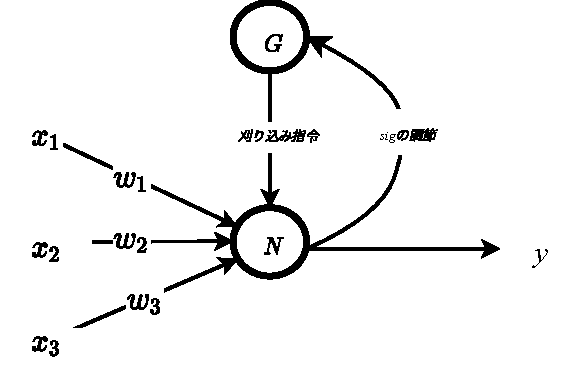
\includegraphics[width=8cm]{NewNeuroGlia.pdf} 
  \caption{Neuro-Glia相互調節機構} 
\end{figure}

\begin{comment}
\begin{figure}[H]
  \begin{minipage}{0.5\hsize}
    \centering
    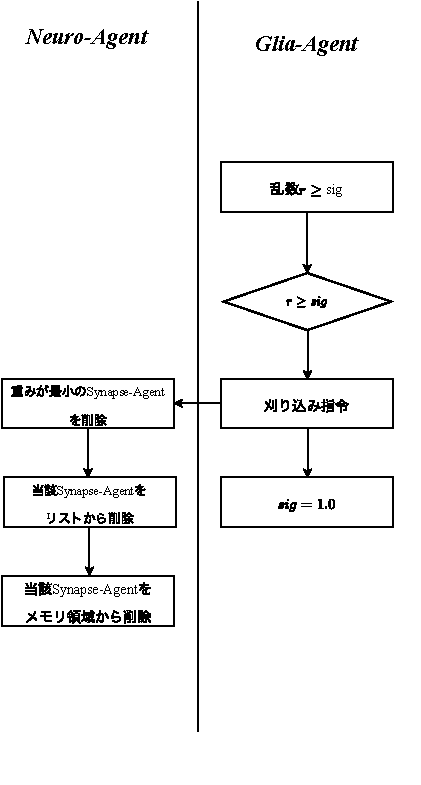
\includegraphics{FlowChartGN.pdf}
    \subcaption{Glia-AgentからNeuro-Agentへの作用:刈り込み}
  \end{minipage}
  \begin{minipage}{0.5\hsize}
    \centering
    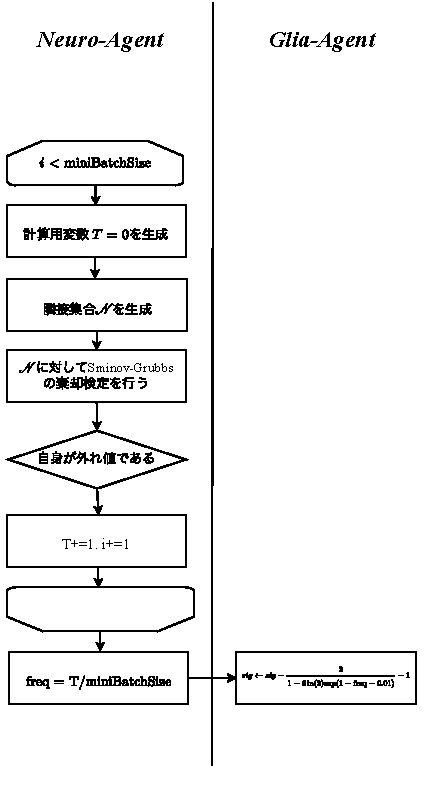
\includegraphics{FlowChartNG.pdf}
    \subcaption{Neuro-AgentからGlia-Agentへの作用:閾値の調節}
  \end{minipage}
  \caption{キャプション}
\end{figure}
\end{comment}
\begin{align}
  Glia.sig\leftarrow Glia.sig-&\displaystyle \cfrac{2}{1+exp((Neuron.freq-0.1))}-1\\
  &k=6\ln(3)
  \label{eq:new}
\end{align}
ここで, NAの活動頻度とは以下のように求める.
\begin{enumerate}
  \item 活動頻度計算用変数$T$を用意する.
  \item エージェント自身を含むクリークにおいて, 
  smirnov-grubbs検定を行う.
  \item 検定の結果, 自身が外れ値であると判断された場合に1, そうでなければ0を$T$に加算する.
  \item 2〜3の工程をミニバッチ分繰り返す.
  \item 以下の式を用いて, 自身の活動頻度が求まる.
  \vspace{-2zh}
  \begin{align}
    Neuron.freq=\cfrac{T}{miniBatchSize}
  \end{align}
\end{enumerate} 
\subsection{グリアネットワーク}
\wsec{g-asem}節に述べた通り, 実際の脳ではミクログリアは単体で
刈り込みを行っているのではなく, 
グリアアセンブリを介して, 協調し全体としての利益に資する行動を
とっているものと見られる.

本モデルはグリアアセンブリの模倣として$GA$同士のネットワークである
グリアネットワークを定義した.
グリアネットワークは, 抑制信号$sig$を他の$GA$に伝播する.
これにより, 時空間的に局所的な刈り込みを抑制し, ネットワークの破綻を防ぐ役割がある.

抑制信号は, グリアネットワーク上の伝播距離(ホップ数)に応じて減衰定数$A$だけ減衰していく.
なお, 複数の距離が与えられた場合, 最も近い$GA$の影響を優先する.
例えば, \wfig{GliaNetworks}の$g_2$の場合, 
$g_0\rightarrow g_1\rightarrow g_2$と$g_0\rightarrow g_2$の経路では後者の経路のみを考えることになる.
\vspace{-3zh}
\begin{figure}[H]
  \centering
  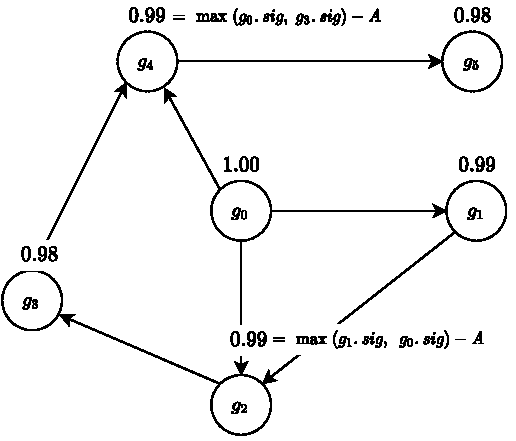
\includegraphics[width=8cm]{GliaNetworks.pdf}
  \caption{グリアネットワークでの抑制信号の伝達}
  \label{fig:GliaNetworks}
\end{figure}
\vspace{-2zh}
\section{計算機実験}
学習タスクとして6bitの入力の上位3bitのいずれかに1が入っているかどうか
の判別を行った出力値は結果が真である確率である. 
その他のパラメータは以下に示す通りである(\wtab{param}).
\begin{table}[H]
  \caption{パラメータ一覧}
  \label{tab:param}
  \centering
   \begin{tabular}{ll}
    \toprule
      パラメータ&値\\\midrule\midrule
      学習率$\eta$&$0.5$\\
      エポック数$Epocs$&$100$\\
      ミニバッチサイズ$miniBatchSize$&$100$\\
      初期ニューロン数$Neurons$&$31$\\
      初期グリア数$Glias$&$31$\\
      初期シナプス数$Mill$&$182$\\
      減衰率$A$&0.01\\
      入力サイズ$Inputs$&$6$\\
      出力サイズ$Outputs$&$1$\\
    \bottomrule
   \end{tabular}
 \end{table}
計算機実験の結果を\wfig{SynapseNum},\wfig{LearningCurve}に示す.
刈り込みを行った結果, 最終的なシナプス数は78に推移した.よって, 削減割合は
57%であり, また, \wfig{LearningCurve}より刈り込みによる精度悪化は認められないため, 
不要なシナプスの剪定が適切に行われたと評価できる.
\begin{figure}[H]
  \centering
  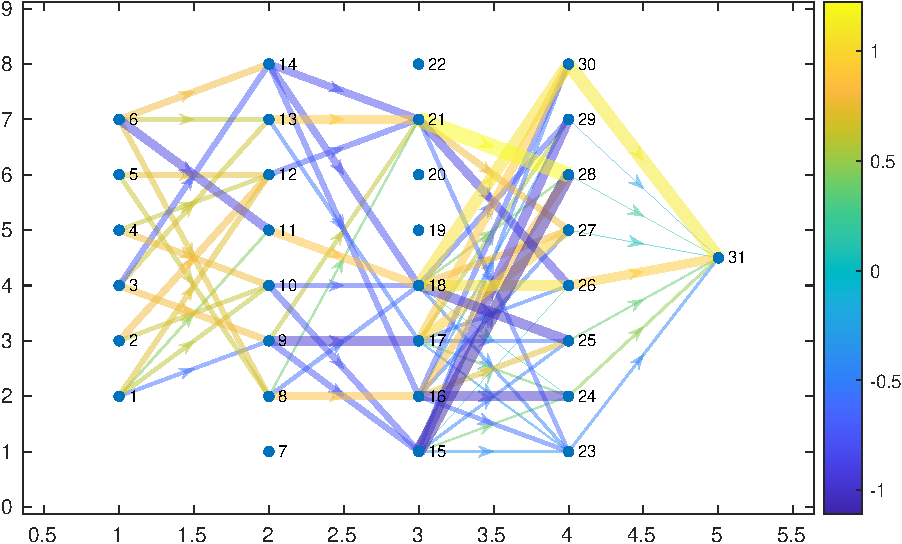
\includegraphics[width=8cm]{Graph-crop.pdf} 
  \caption{刈り込み後のネットワーク}
  \label{fig:Graph}
\end{figure}
\vspace{-2zh}
\begin{figure}[H]
  \centering
  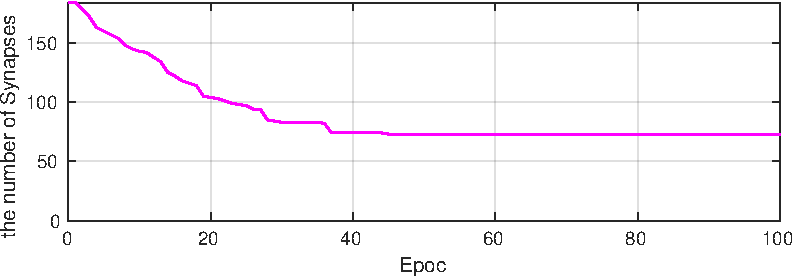
\includegraphics[width=8cm]{SynapseNum-crop.pdf} 
  \caption{シナプス量の変化}
  \label{fig:SynapseNum}
\end{figure}
\vspace{-2zh}
\begin{figure}[H]
  \centering
  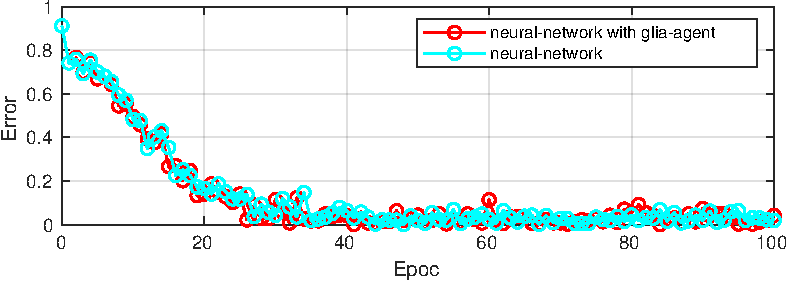
\includegraphics[width=8cm]{LearningCurve-crop.pdf} 
  \caption{学習曲線}
  \label{fig:LearningCurve}
\end{figure}
 
\section{結論}
グリア細胞に着想を得た監視エージェントを導入することによって
全体の管理者のいないMASに対応した
ニューラルネットワークの学習パラメータの削減を行うことができた.
このパラメータの削減にあたっては, 学習精度の悪化が認められなかったことから, 
刈り込みが適切に行われたものと評価できる
一方で, グリアネットワークの構造依存性や
MASに特有な問題(合意制御, 環境認識), あるいは畳み込みのMAS化など
実用化にあたっては
さらなる発展が必要である.
 \begin{thebibliography}{99}
  \bibitem{Neuron-Glia} 	
野村靖幸,北海道大学,神経免疫相関とくにニューロン・グリア相互作用機構に関する分子薬理学的研究, \url{https://kaken.nii.ac.jp/ja/grant/KAKENHI-PROJECT-06454595/}
  \bibitem{Tensorizing}
  Novikov, Alexander, et al. "Tensorizing neural networks." Advances in neural information processing systems 28 (2015).
  \bibitem{次数重み付き平均法}
  原田和明, 右田剛史, and 高橋規一.``ニューラルネットワークの分散学習における新たな合意重み決定法.'' IEICE Conferences Archives. The Institute of Electronics, Information and Communication Engineers, 2019.
\end{thebibliography}
 \end{document}
